\documentclass[11pt,class=report,crop=false]{standalone}
\usepackage[screen]{../mathgame}


\begin{document}


%====================================================================
\chapitre{Sociologie du joueur}
%====================================================================

%
%\insertvideo{yUgpElITYTg}{partie 5.1. Bits classiques}
%
%\insertvideo{iET0snUXj0k}{partie 5.2. Portes logiques}
%
%\insertvideo{JKmC2u5kvKg}{partie 5.3. Algorithme et complexité}


\objectifs{Quel est le comportement d'un joueur dans la \og{}vraie vie\fg{} et quels sont les paramètres qui permettent de créer un \og{}bon\fg{} jeu ?}


%%%%%%%%%%%%%%%%%%%%%%%%%%%%%%%%%%%%%%%%%%%%%%%%%%%%%%%%%%%%%%%%%%%%%
\section{Jeu réel}

Aux échecs la meilleure stratégie est rationnelle. Il y a peu de chance que vous battiez un bon joueur en jouant certains coups au hasard ou selon votre humeur. Cependant, dans des jeux moins rationnels, le comportement humain n'est pas toujours celui que l'on attend. Le poker ou le black jack sont des exemples de jeux avec une forte part de hasard, mais il existe une stratégie rationnelle qui tient compte des probabilités en fonction des cartes découvertes et celles que vous avez en main.
Cette stratégie ne vous garantit pas de gagner mais vous assure la meilleure \emph{espérance} de gain, c'est-à-dire le meilleur gain possible si vous pouviez répéter l'expérience de nombreuses fois. Par exemple si je joue à pile ou face avec une pièce truquée qui tombe sur \og{}pile\fg{} deux fois sur trois, alors la meilleure stratégie est bien évidemment de choisir \og{}pile\fg{}, cela ne m'assure pas de gagner à tous les coups, mais si je joue $1000$ fois, je devrais gagner environ 666 fois. Nous allons voir que pour certains jeux le comportement humain n'est pas toujours le plus rationnel.

%--------------------------------------------------------------------
\subsection{Jeu de l'ultimatum}

\textbf{Le jeu.}
Le \defi{jeu de l'ultimatum} est un jeu à deux joueurs : le \emph{proposant} et le \emph{répondant}. On met à disposition du proposant une certaine somme d'argent (disons $100$ euros), il doit faire une offre de partage à l'autre joueur (ex. \og{}je te donne $20\%$ de mes $100$ euros\fg{}). Le répondant a deux possibilités :
\begin{itemize}
	\item Il accepte l'offre (et alors le partage se fait selon la répartition convenue).
	\item Il refuse l'offre et alors \emph{personne} ne gagne rien.
\end{itemize}

Le proposant et le répondant ne peuvent pas négocier, c'est une situation \og{}à prendre ou à laisser\fg{} pour le répondant.

Voici l'arbre du gain du répondant, pour une somme initiale $S$ et une proposition de pourcentage $p$.

\myfigure{1}{
	\tikzinput{socio-01}
} 

\medskip

\textbf{Solution rationnelle.}
La seule stratégie rationnelle pour le répondant c'est d'accepter la proposition quelle soit ! En effet, en acceptant l'offre, il a un gain positif ou nul, toujours supérieur ou égal au gain nul s'il refuse.
Sachant cela, la stratégie rationnelle du proposant serait d'offrir un pourcentage le plus petit possible (voire même $0$).

\medskip

\textbf{Expérimentations.}
De nombreuses expériences de ce jeu ont été réalisées dans différents pays avec différentes cultures. Voici ce qui en ressort :
\begin{itemize}
	\item Le proposant soumet généralement une part de la somme comprise entre 40\% et 50\%. Lorsque le répondant est de la même communauté que le proposant (famille, amis, même village) alors le pourcentage proposé est généralement 50\%.
	
	\item Les offres de 40\% et plus sont généralement acceptées par les répondants.

	\item Les offres de 20\% et moins sont généralement refusées (avec une offre à 20\%, environ 50\% de rejet, avec une offre à 10\% environ 90\% de rejet).
\end{itemize} 

C'est ce dernier point qu'il convient d'expliquer car du point de vue d'un bilan purement comptable, le répondant a tout simplement refusé de l'argent !
Les explications de ce refus avancées par les répondants sont :
\begin{itemize}
	\item donner une leçon (au cas où la situation se répéterait dans le futur),
	\item punir (car le répondant trouve l'offre injuste et en souffre).
\end{itemize}

Cette expérience met en avant le besoin d'équité et de justice pour vivre en société.

Les expérimentations ont été menées avec des petites sommes (disons de 10 à 100 euros), pour des sommes plus élevées, on peut penser que les résultats seraient différents. Par exemple refuseriez-vous ma proposition de 10\% de 1\,000\,000 d'euros ?
Le jeu serait aussi différent s'il était répété plusieurs fois de suite (ou si on échangeait de rôle une fois sur deux). Voir le jeu \emph{tit-for-tat} du chapitre \og{}Théorie des jeux\fg{}.


\medskip
Dans le jeu de l'ultimatum, le répondant a intérêt à être égoïste et à garder le maximum d'argent pour lui en espérant que son offre soit acceptée. Dans le jeu suivant la situation est renversée : le joueur a intérêt à être le plus généreux possible.

%--------------------------------------------------------------------
\subsection{Jeu à contribution}


\textbf{Le jeu.}
Voici comment jouer au \defi{jeu à contribution} :
\begin{itemize}
	\item il y a $n$ joueurs,
	\item chaque joueur reçoit la même somme $S$,
	\item chaque joueur décide secrètement de placer tout ou partie de sa somme dans le pot commun. Il garde pour lui le reste.
	\item La somme totale $S$ du pot commun est multipliée par un facteur $k$ (avec $1 < k < n$) : $S'= k \times S$.
	\item Le montant du pot commun revalorisé est réparti équitablement entre les $n$ joueurs ($S'/n$).
	\item À la fin, chaque joueur dispose donc de l'argent qu'il n'a pas mis au pot, auquel s'ajoute le partage du pot commun revalorisé.
\end{itemize}

%\bigskip
%
%\textbf{Formule.}
%
%\begin{itemize}
%	\item Notons $s_i$ la somme que le joueur $i$ place dans le pot commun somme  ; il garde le reste $S-s_i$ dans sa cagnotte.
%	\item Le total du pot commun est donc $\sum_{i=1}^n s_i$.
%	\item Le pot commun revalorisé est $k\sum_{i=1}^n s_i$.
%	\item Ce qui fait pour chacun $\frac{k}{n}\sum_{i=1}^n s_i$.
%	\item Ainsi le joueur $i$ possède à la fin un total de :
%	$$S-s_i + $\frac{k}{n}\sum_{i=1}^n s_i.$$
%\end{itemize}	
%	

\bigskip

\textbf{Exemple.}


\myfigure{1}{
	\tikzinput{socio-02}
} 

Prenons $n=4$ joueurs qui disposent chacun de $S=100$ avec un facteur multiplicatif qui est $k=1.2$.
Chacun décide de mettre respectivement 40, 100, 0, 80 dans le pot commun.
Le total du pot est donc 220, qui une fois revalorisé est $k \times 220 = 264$.
Le pot revalorisé est réparti en parts de 66 euros entre les quatre joueurs.
À la fin :
\begin{itemize}
	\item le joueur 1 a $60+66 = 126$ (les 60 qu'il n'a pas partagés et sa part du pot commun), 
	\item le joueur 2 a $0+66 = 66$,
	\item le joueur 3 a $100+66 = 166$,
	\item le joueur 4 a $20+66 = 86$.			
\end{itemize} 

\medskip

\textbf{Meilleure stratégie.}
La meilleure stratégie collective c'est que tout le monde mette tout son argent au pot commun afin de profiter au maximum du facteur $k$. Dans l'exemple précédent les joueurs ont à la fin un total de 444 euros alors que s'ils avaient tout mis au pot commun ils se seraient partagés 480 euros (120 chacun).

Cependant ce qui peut arriver de mieux pour un joueur précis, c'est qu'il ne mette rien au pot commun mais que tous les autres donnent tout. Dans la situation précédente avec quatre joueurs, le joueur égoïste obtiendrait 190 euros et les autres 90 euros chacun.

L'impôt est une analogie de la vie courante : tout le monde paye des impôts et en échange profite des écoles, des routes\ldots{} mais si une personne se débrouille pour ne pas en payer, elle profite à la fois de son argent pas dépensé et des infrastructures !

\medskip

\textbf{Expérimentations.}
Dans la pratique, les joueurs ont tendance à placer quelque chose dans le pot : une somme variant de 0 à 100\% de la somme possible (mais rarement 0) et qui dépend aussi du facteur $k$. 
Les pourcentages se stabilisent si le jeu est répété, les joueurs ont tendance à baisser leur contribution lorsqu'ils s'aperçoivent que d'autres ont été moins généreux. Par exemple, avec un facteur $k=1.3$, le pourcentage placé au pot commun est environ de $50\%$.


%--------------------------------------------------------------------
\subsection{Partage de Shapley}

\index{formule!du partage de Shapley}

Dans les jeux coopératifs (ou dans la vraie vie) chacun fournit une contribution plus ou moins importante. Si le groupe gagne une somme $S$, comment répartir les gains de façon équitable en tenant compte de la participation de chacun ? 
Une formule possible est donnée par le \defi{partage de Shapley} du nom de Lloyd Shapley (1923--2016), mathématicien qui a obtenu la récompense dite \og{}prix Nobel d'économie\fg{} pour ses travaux.

\bigskip

\textbf{Fonction valeur.}

Le jeu se joue à $n$ joueurs numérotés de $1$ à $n$. On attribue un gain à chaque groupe de joueurs à l'aide d'une fonction $v$.

\begin{itemize}
	\item On note $v(1)$, $v(2)$, \ldots, $v(n)$ le gain obtenu par un joueur s'il jouait tout seul. Les joueurs ne sont pas nécessairement tous du même niveau, et donc les gains individuels peuvent être différents.
	
	\item On note  $v(i,j)$ le gain de la coalition des deux joueurs $i$ et $j$.
	 Ainsi $v(1,2)$ est le gain obtenu par le regroupement des joueurs $1$ et $2$.
	 
	\item Plus généralement si $E$ est sous-ensemble de $\{1,2,\ldots,n\}$ alors $v(E)$ désigne le gain de la coalition des joueurs de $E$. Exemple : $v(1,3,4)$ est le gain obtenu lorsque les joueurs $1$, $3$ et $4$ se regroupent.
	
	\item On note $S= v(1,2,\ldots,n)$ le gain obtenu par le groupe tout entier. C'est cette somme qu'il faut maintenant partager équitablement entre tous les joueurs.
	
	\item Par définition $v(\varnothing)=0$ (où $\varnothing$ est l'ensemble vide, avec $\Card \varnothing = 0$).
		
\end{itemize}

\bigskip

\textbf{Hypothèse.}
Nous supposons que la fonction $v$ est \defi{sur-additive}, c'est-à-dire :
$$v(E \cup F) \ge v(E) + v(F),$$
pour toutes parties $E$ et $F$ de $\{1,\ldots,n\}$ qui sont disjointes (c'est-à-dire 
$E \cap F = \varnothing$).
Cela signifie que les joueurs de $E$ et $F$ réunis ensemble gagnent plus (ou autant) que la somme des gains de la coalition de $E$ avec les gains de la coalition de $F$. Les joueurs ont donc intérêt à se réunir.

\bigskip

\textbf{Formule de Shapley.}

Voici une formule qui permet de répartir les gains $\sigma_i$ en tenant compte de la valeur de chaque joueur $i$ (plus le joueur $i$ est important, plus son gain $\sigma_i$ sera grand). La formule nécessite de connaitre le gain $v(E)$ pour n'importe quel sous-ensemble $E$ de $\{1,\ldots,n\}$.

\mybox{$\displaystyle
\sigma_{i_0} = \frac1n \sum_{\substack{E \subset \{1,\ldots,n\}\\\text{t.q. } i_0 \notin E}} \binom{n-1}{\Card E}^{-1} \big(	v(E \cup \{ i_0 \}) - v(E) \big)
	$}
La formule est délicate à comprendre et on verra des exemples juste après.
Notons que :
\begin{itemize}
	\item $v(E \cup \{ i_0 \}) - v(E)$ est le bénéfice de voir $i_0$ rejoindre la coalition $E$,
	\item la formule est une moyenne (pondérée) de tous ces bénéfices et prenant tous les sous-ensembles $E$ de $\{1,\ldots,n\}$ ne contenant pas $i_0$ (il ne faut pas oublier $E=\varnothing$ parmi ceux-ci).
	\item Rappelons que $\Card E$ est le \defi{cardinal} de l'ensemble $E$, c'est-à-dire son nombre d'éléments.
	\item $\binom{p}{k}$ est le \defi{coefficient binomial} appelé aussi \defi{$k$ parmi $p$} et se calcule par la formule :
	$$\binom{p}{k} = \frac{p!}{k!(p-k)!}.$$
	Ainsi :
	$$\binom{p}{0} = 1 \qquad
	\binom{p}{1} = p \qquad
	\binom{p}{2} = \frac{p(p-1)}{2} \qquad \cdots \qquad \binom{p}{p} = 1
	$$
\end{itemize} 


\bigskip

\textbf{Exemples à deux joueurs.}

Pour $n=2$ la somme à partager est $S=v(1,2)$. Les gains de chacun sont :
$$
\sigma_1 = \frac12\big( v(1,2) + v(1) - v(2)\big)
\qquad\qquad
\sigma_2 = \frac12\big( v(1,2) + v(2) - v(1)\big)
$$

Preuve pour $\sigma_1$ : les ensembles de $\{1,2\}$ qui ne contiennent pas $1$ sont $E=\varnothing$ (de cardinal $0$, avec $v(\varnothing)=0$) et $E = \{2\}$ (de cardinal $1$) donc la formule de Shapley donne :
$$
\sigma_1 
= \frac12\Bigg(
\  
\underbrace{\binom{1}{0}^{-1} \left( v(1) - 0\right)  }_{\text{cas } E=\varnothing} 
\ 
+ \  \underbrace{\binom{1}{1}^{-1} \left(	v(1,2) - v(2) \right)}_{\text{cas } E=\{2\}}  
\ \Bigg) 
= \frac12\big( v(1,2) + v(1) - v(2) \big)$$

Voici un exemple concret : supposons $v(1) = 4$, $v(2)= 2$, et pour les deux joueurs réunis $v(1,2) = 10$ (ainsi $v(1,2) \ge v(1)+v(2)$ comme requis pour la formule).
Comment les joueurs se partagent le gain $S=10$ obtenu en commun ?
La formule de Shapley donne :
$$\sigma_1 = \frac12(10 + 4 -2) = 6 
\quad \text{ et } \quad 
\sigma_2 = \frac12(10 + 2 -4) = 4$$
Ainsi même si le joueur 1 est individuellement deux fois plus fort que le joueur 2, il n'obtient pas deux fois plus que le joueur 2, en effet il a eu besoin du joueur 2 pour partager une plus forte somme qu'il n'aurait pas pu obtenir tout seul.


Terminons avec un autre exemple : un patron (joueur 1) et un employé (joueur 2). L'employé ne peut pas travailler si le patron n'est pas là. Ainsi la fonction valeur est la suivante :
$$v(1) = 1 \qquad v(2) = 0 \qquad v(1,2) = 2$$
La formule de Shapley nous donne $\sigma_1 = \frac32$ et $\sigma_2 = \frac12$. Ainsi la patron récupère 75\% des bénéfices et donne 25\% à l'employé. Noter que l'on n'est pas loin du pourcentage considéré comme acceptable dans le jeu de l'ultimatum.

\bigskip

\textbf{Exemples à trois joueurs.}

La formule de partage pour trois joueurs est :

$$\sigma_1 = \frac16\big(
2v(1,2,3) + v(1,2) + v(1,3) + 2v(1) - 2v(2,3)-v(2)-v(3)
\big)$$
$$\sigma_2 = \frac16\big(
2v(1,2,3) + v(1,2) + v(2,3) + 2v(2) - 2v(1,3)-v(1)-v(3)
\big)$$
$$\sigma_3 = \frac16\big(
2v(1,2,3) + v(1,3) + v(2,3) + 2v(3) - 2v(1,2)-v(1)-v(2)
\big)$$

À vous de vérifier ces formules, par exemple pour calculer $\sigma_1$ on considère les ensembles $E$ ne contenant pas $1$ : ce sont $\varnothing$, $\{2\}$, $\{3\}$, $\{2,3\}$.

\medskip

Considérons un exemple à trois joueurs avec $v(1)=1$, $v(2)=2$ et $v(3)=3$.
Supposons que lorsque les joueurs forment un groupe alors les gains s'ajoutent (la fonction $v$ est additive $v(E \cup F) = v(E)+v(F)$, par exemple $v(1,3) = v(1)+v(3) = 4$ et $v(1,2,3)=v(1)+v(2)+v(3) = 6$). Il n'y a donc pas de bonus à se regrouper. Vérifier que, dans ce cas, chacun récupère un gain selon sa valeur individuelle : $\sigma_1 = 1$, $\sigma_2 = 2$, $\sigma_3 = 3$.

\medskip

Considérons l'exemple avec les données suivantes :
$$v(1) = 1 \quad v(2) = 2 \quad v(3) = 0
\quad v(1,2) = 4 \quad v(1,3) = 2 \quad v(2,3) = 4 \quad v(1,2,3) = 10$$
Alors 
$$\sigma_1 = 3 \qquad \sigma_2 = 4.5 \qquad \sigma_3 = 2.5$$
Noter que dans cet exemple le joueur 3 n'obtient aucun gain individuellement mais qu'il apporte une contribution lorsqu'il est en groupe. Noter aussi aussi que le fait de se regrouper apporte un bonus notable.

\medskip

Terminons avec un patron fainéant (qui ne produit pas) et ses deux employés (qui ne produisent qu'en sa présence) :
$$v(1)=0  \quad v(2) = 0 \quad v(3) = 0
\quad v(1,2) = 1 \quad v(1,3) = 1 \quad v(2,3) = 0 \quad v(1,2,3) = 2$$
Alors 
$$\sigma_1 = 1 \qquad \sigma_2 = \frac12 \qquad \sigma_3 = \frac12$$
Ainsi le patron fainéant récupère la moitié des gains.
On retrouve ce résultat plus généralement pour un patron fainéant et $k$ employés : le patron récupère la moitié des gains et ses employés se partagent l'autre moitié.



%%%%%%%%%%%%%%%%%%%%%%%%%%%%%%%%%%%%%%%%%%%%%%%%%%%%%%%%%%%%%%%%%%%%%
\section{Qu'est-ce qu'un \og{}bon\fg{} jeu ?}

Un bon jeu c'est de l'amusement et de l'engagement ! Voyons quelques paramètres pour créer un tel jeu.

%--------------------------------------------------------------------
\subsection{Courbe d'apprentissage}

\index{courbe!d'apprentissage}

Nous allons voir différentes façons de décrire l'apprentissage d'un joueur.

\myfigure{1.1}{
	\tikzinput{socio-03}
}

En abscisse nous notons \og{}temps\fg{} parce que c'est le principal facteur d'apprentissage : la durée passée à apprendre. Ce n'est pas toujours vrai (par exemple si on est tout seul, on peut apprendre de travers). On pourrait parler d'\og{}expérience\fg{} mais ce mot reste ambigu.
En ordonnée nous avons la \og{}maîtrise\fg{}, cela pourrait aussi être la \og{}connaissance\fg{} ou bien le \og{}niveau\fg{} atteint. Cette valeur peut être limitée ou pas.
Une analogie économique serait la courbe des \og{}profits\fg{} (ordonnée) en fonction de l'\og{}investissement\fg{} (abscisse).

Voici différents modèles de courbes d'apprentissage.

\myfigure{1}{
	\tikzinput{socio-04}
}
\myfigure{1}{
	\tikzinput{socio-05}
}


On peut distinguer les courbes qui sont bornées (sur la première ligne des figures précédentes) ou non (sur la seconde ligne).
On peut aussi distinguer les apprentissages à feedback positif ou négatif.
Une évolution à feedback positif : plus j'avance, plus mon niveau augmente vite. Ce sont des courbes qui croissent plus vite qu'une fonction linéaire (c'est par exemple le cas avec une courbe exponentielle). Par exemple, au monopoly si j'ai peu de propriétés je gagne peu d'argent, mais si j'ai beaucoup de propriétés je gagne beaucoup beaucoup d'argent et je peux acheter davantage de propriétés. Une évolution peut aussi être à feedback négatif : plus j'avance plus les niveaux sont difficiles à atteindre. Par exemple : je termine un niveau, mais le niveau suivant sera plus dur, ou alors je doit atteindre le même objectif mais avec moins de ressources. C'est par exemple le cas pour la progression d'une armée (réelle ou virtuelle), plus elle s'enfonce en territoire ennemi, plus sa progression est difficile (ravitaillement, communication, connaissance du terrain\ldots).


Dans la vie réelle, l'apprentissage (par exemple de la conduite d'une voiture) connait des périodes de stagnation (voire de régression) :
\myfigure{1}{
	\tikzinput{socio-06}
}


La notion de courbe d'apprentissage ne concerne pas que les humains. 
Les ordinateurs aussi apprennent : par exemple à distinguer un chat d'un chien sur une photo, à jouer aux échecs et à piloter des voitures. Pour cela il s'agit d'entraîner un \og{}réseau de neurones\fg{} en lui montrant par exemple 1000 images de chiens et 1000 images de chats (et en lui disant qui est qui). Ce processus est itéré plusieurs fois avec les mêmes images. Ensuite un réseau de neurones bien entraîné saura reconnaitre de nouvelles images.
Voici typiquement la courbe d'apprentissage : elle mesure le taux de succès (par exemple reconnaissance correcte de chat vs chien sur des \emph{nouvelles} images) en fonction de la longueur d'apprentissage (on parle d'\og{}époques\fg{}) (par exemple le nombre d'images soumises, sachant qu'une fois les 2000 images épuisées on recommence avec la première image).

\begin{center}
	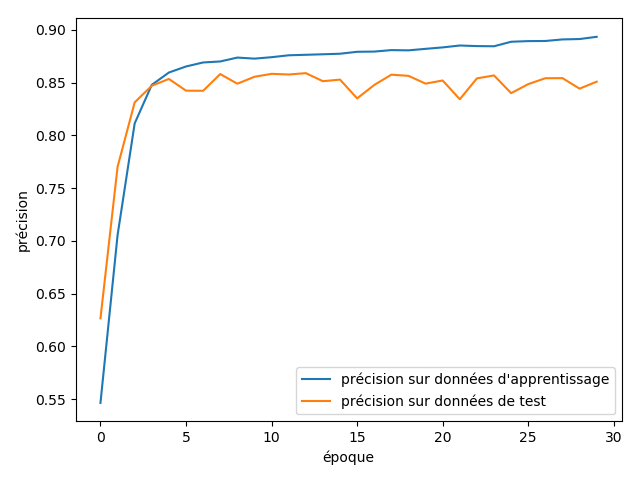
\includegraphics[scale=\myscale,scale=0.6]{figures/socio-deepmath}
\end{center}

La précision sur les données d'apprentissage augmente et finit par plafonner.
Sur les données de test la précision augmente aussi puis l'apprentissage ne sert plus à rien et la précision peut même diminuer.
Que se passe-t-il ? C'est un phénomène de sur-apprentissage. Le réseau de neurones a fini par apprendre par c\oe ur les données d'entraînement mais n'est plus efficace sur les données nouvelles (comme un étudiant qui apprend par c\oe ur les solutions de la feuille d'exercices sans comprendre: il n'arrivera pas à faire les exercices inédits le jour de l'examen !).

%--------------------------------------------------------------------
\subsection{Jeu gagnable}

Un bon jeu se doit d'être \og{}gagnable\fg{} et \og{}équitable\fg{}.

\textbf{Gagnable.} 
\begin{itemize}
	\item Le jeu doit être perçu comme gagnable, ceci quelle que soit la progression du joueur dans le jeu. 
	\item On peut découper le jeu en niveaux afin de proposer des gains partiels et des récompenses intermédiaires. 
	\item Le joueur doit sentir qu'il progresse vers l'objectif. 
	\item Un joueur expérimenté doit avoir plus de chance de gagner.
	\item Le jeu doit pouvoir être gagné même en cas d'une erreur du joueur au début de la partie.
\end{itemize}

\medskip

\textbf{Pas trop facile.}
\begin{itemize}
	\item Un jeu ne doit pas être trop facile, sinon il perd de son intérêt.
	\item Cependant les débuts doivent être faciles pour éviter de décourager le joueur.
	\item Les jeux toujours faciles et à priori sans intérêt peuvent avoir du succès, ils permettent par exemple de se vider la tête ou de s'occuper sans réfléchir.
\end{itemize}

\medskip

\textbf{Illusion de gagnabilité.}
\begin{itemize}
	\item Le jeu doit paraître gagnable mais ne l'est pas forcément.
	Autrement dit, même s'il est très rarement possible de gagner, le joueur doit toujours penser que c'est possible.
	
	\item Un bon exemple est ce jeu de fête foraine dans lequel on glisse des pièces qui entraînent d'autres pièces qui sont censées finir par tomber par gros paquets, mais où en fait on ne récupère au mieux que quelques pièces.
	
	\item Un autre exemple est le loto. Si le loto était présenté comme un tirage d'un numéro entre un et dix millions, personne ne jouerait. Mais avec le système à plusieurs numéros, le joueur va régulièrement obtenir un ou plusieurs bons numéros, voire des numéros proches des bons, ce qui lui fera penser qu'il n'était pas loin de gagner (notion qui n'a pas de sens ici !). De plus la loterie médiatise fortement les succès des gagnants pour obtenir un effet \og{}pourquoi pas moi ?\fg{}	
\end{itemize}

%--------------------------------------------------------------------
\subsection{Jeu équitable}

\textbf{Équité.}

Que le jeu soit un jeu de :
\begin{itemize}
	\item \emph{compétence} (échec, course de voitures, jeu de tir\ldots), 
	\item \emph{patience} (dressage d'animaux, gestion d'une ferme, peinture au numéro\ldots),
	\item \emph{chance} (loterie, casino\ldots),
\end{itemize}
alors ce jeu doit être équitable.

Voici la définition de \og{}équité\fg{} dans le Larousse :
\begin{quote}
	\defi{Équité} : Qualité consistant à attribuer à chacun ce qui lui est dû par référence aux principes de la justice naturelle. 
\end{quote}	
Il ne faut pas confondre \emph{équité} et \emph{égalité} : il semble normal lors d'une récompense d'attribuer une plus grande part au plus gros contributeur de la réussite.

\medskip

\textbf{Ressources.}

\begin{itemize}
	\item Les ressources (objets, pouvoirs, terrain, argent, temps\ldots) doivent être partagées de façon équitable (ou même égale) entre les joueurs.
	
	\item Une façon de réaliser ceci est par symétrie du jeu. Par exemple aux échecs les deux joueurs ont les mêmes pièces avec les mêmes mouvements. La seule petite asymétrie (très importante pour les grands joueurs) est que le joueur avec les pièces blanches commence. Ce défaut de symétrie est réparé sur plusieurs parties en alternant celui qui débute la partie.
	
	\item Pour les jeux asymétriques on peut rétablir l'équilibre par des relations de non-transitivité.
	Rappelons qu'une relation est \emph{transitive} si $a\mathcal{R}b$ et $b\mathcal{R}c$ implique $a\mathcal{R}c$ (exemple : si $a\le b$ et $b\le c$ alors $a\le c$). Exemple de relation non-transitive : les joueurs peuvent choisir entre  trois personnages $A$, $B$ ou $C$ qui ont chacun des pouvoirs différents. Pour que le jeu soit intéressant il ne faut pas qu'un personnage soit plus fort que tous les autres. Il faut par exemple que $A \ge B$, $B \ge C$ mais $C \ge A$. C'est le cas dans le jeu \og{}pierre/feuille/ciseau\fg{}, \og{}poules/renards/vipères\fg{} ou pour les cartes \emph{Pokémon}.
	
	\item Le ratio coût/avantage des objets doit être bien dosé. Exemple : obtenir un super-pouvoir doit demander de battre un monstre vraiment méchant. 
	
	\item Les ressources doivent être méritées si elles ne sont pas partagées équitablement. Exemple : l'achat intégré d'un joli costume pour un avatar ne pose pas de problème, par contre l'achat d'une super-arme qui permet de tout gagner est mal venu.
\end{itemize}

\medskip

\textbf{Niveau.}

\begin{itemize}
	\item Un joueur plus expérimenté doit avoir plus de chance de gagner.
	
	\item Pour conserver le plaisir de jouer on peut regrouper les joueurs par poules de niveau équivalent.

	\item Si on décide de jouer une partie avec des joueurs de différents niveaux, alors on peut attribuer un \emph{handicap} aux meilleurs joueurs. Par exemple les meilleurs chevaux d'une course hippique sont chargés d'un poids supplémentaire.
 	Au contraire on peut aussi favoriser les joueurs les moins bons. Par exemple au go, le joueur le moins bon a des pierres supplémentaires au départ ; à \emph{Mario Kart} le dernier de la course trouve sur sa route des boîtes qui contiennent des avantages conséquents qui lui permettent de revenir dans la course.
 	
\end{itemize}
\medskip

\textbf{Contrôle.}

\begin{itemize}
	\item Les décisions du joueur doivent être déterminantes pour l'issue du jeu.
	
	\item Par exemple si vous devez choisir entre le chemin de gauche contre un monstre ou celui de droite vers un lac paisible cela doit avoir une conséquence pour la suite du jeu (par exemple gain d'expérience, perte de vie, chemins ultérieurs possibles\ldots). Cependant aucun choix (surtout en début de partie) ne devrait empêcher de gagner la partie.

\end{itemize}

\medskip

\textbf{Chance.}

\begin{itemize}
	\item Le hasard c'est lorsque le joueur n'a pas de contrôle sur l'issue de l'aléa.
	
	\item Un jeu de hasard ou avec une part de chance peut quand même être un jeu équitable, mais sous certaines conditions. 
	
	\item Le gain, ainsi que la probabilité de le gagner, doivent être connus du joueur. Par exemple, pour atteindre la rue de la Paix je dois faire 7 avec deux dés : je sais que j'aurai une chance sur six. De même au loto ou au casino le jeu est considéré comme équitable car le gain et la probabilité de gagner sont publics (en fait le loto et le casino redistribuent entre 50\% et 95\% des mises).
	
	\item Un exemple de ce qui n'est pas équitable peut être des \emph{loot boxes} (ce sont des boîtes surprises que l'on peut acheter au cours du jeu). Le joueur ne sait pas toujours s'il va obtenir un nouveau costume pour son avatar (sans intérêt) ou bien une nouvelle arme (qui le rend plus puissant).
	
	\item Un jeu peut avoir une part de chance sous la forme :
	\begin{itemize}
		\item un peu de hasard de façon assez fréquente,
		\item un gros aléa mais qui se produit rarement.
	\end{itemize}
On peut aussi laisser le choix au joueur de faire intervenir le hasard : \og{}payer une amende de 100 euros ou bien tirer une carte chance\fg{}.
	
	\item Lorsqu'il est crucial pour le jeu, le hasard devrait être \emph{certifié}.
	C'est particulièrement important pour les jeux d'argent en ligne (poker, black jack, roulette\ldots) : le joueur doit être sûr que le tirage est vraiment aléatoire. On peut utiliser un générateur éprouvé de nombres pseudo-aléatoires pour lequel les différents tirages n'ont aucun lien entre eux.
	
\end{itemize}

\bigskip
\textbf{Lois.}

Terminons par deux types de lois qui permettent de générer du hasard :
\begin{itemize}
	\item la \defi{loi uniforme}\index{loi!uniforme} : par exemple chaque nombre entre $a$ et $b$ a autant de chance que les autres d'être choisi (exemple : tirage du loto) ;
	\item la \defi{loi normale}, dite aussi \defi{loi de Gauss}\index{loi!de Gauss} ou \defi{courbe en cloche}, pour laquelle les valeurs autour d'une valeur $\mu$ ont plus de chance d'être choisies que les valeurs éloignées. C'est par exemple la situation de la somme de deux dés (ou la plus forte probabilité est d'obtenir 7 alors qu'obtenir 12 est moins probable), ou la taille d'un homme choisi au hasard dans la population\ldots
\end{itemize}



La densité de probabilité pour la loi uniforme sur $[a,b]$ est la fonction définie par $f(x) = \frac{1}{b-a}$.
	
\myfigure{0.7}{
	\tikzinput{socio-07}
}	

La densité de probabilité de la loi loi normale d'espérance $\mu$ et d'écart-type $\sigma$ est :
	$$f(x) = \frac{1}{\sqrt{2\pi\sigma^2}} \exp\left( -\frac12 \frac{(x-\mu)^2}{\sigma^2} \right)$$
\myfigure{0.6}{
	\tikzinput{socio-08} \quad
	\tikzinput{socio-09}	
}	
Sur la figure de gauche, on représente le graphe de $f$ pour une valeur donnée de $(\mu,\sigma)$ ; la densité de probabilité diminue lorsqu'on l'on s'éloigne de $\mu$ ; l'aire sous la courbe vaut $1$.
Sur la droite sont tracés les graphes de densité de probabilité de la loi normale pour une même valeur de $\mu$ mais avec différentes valeurs $\sigma$ qui mesurent l'étalement de la courbe.


%--------------------------------------------------------------------
\subsection{Candy Crush}

Détaillons quelques aspects d'un jeu à succès : \emph{Candy Crush}.
Ceux qui ne connaissent pas peuvent le tester avant de lire la suite, mais attention de ne pas devenir accro !
On résume ici l'étude \emph{Deconstructing Candy Crush: what instructional design can learn from game design} par E.~Varonis et M.~Varonis (\emph{International Journal of Information and Learning Technology}, 2015).

\textbf{A. Structure du jeu.}

\begin{enumerate}
	\item \textbf{Alignement de bonbons.}	
	\begin{itemize}
		\item Le joueur doit intervertir deux pièces du jeu (des bonbons colorés) afin d'en aligner trois du même type qui vont alors être retirés de la grille. Les bonbons situés au-dessus descendent d'un cran, créant éventuellement d'autres alignements\ldots{} Un alignement de quatre bonbons ou plus crée un bonbon spécial.
		
		\item Ce jeu est joué chaque jour par des millions de personnes dans le monde. Même s'il est gratuit, il produit de très gros bénéfices via des achats intégrés.
	\end{itemize}
	
	\item \textbf{Jeu accessible et addictif.}	
	\begin{itemize}
		\item \emph{Candy Crush} est jouable n'importe où, n'importe quand : il est multi-plateformes et réussir un niveau prend quelques minutes.
		
		\item L'univers bienveillant ramène à l'enfance. Les couleurs sont vives, les enchainements d'explosions en cascades sont inattendus. 
	\end{itemize}
		
	\item \textbf{Niveaux.}	
	\begin{itemize}
		\item Le jeu est découpé en niveaux (plus de $10\,000$) regroupés en épisodes. La carte de progression n'affiche que quelques prochains niveaux pour ne pas étourdir le joueur par l'ampleur du chemin.
		
		\item Chaque niveau a un objectif clair parmi plusieurs possibilités (atteindre un score, faire disparaître de la gélatine, faire tomber certains bonbons\ldots). Le nombre de coups est limité (de façon bien dosée).
		
		\item Les niveaux sont de difficulté croissante. Il n'y a pas de limite pour recommencer un niveau (à condition de patienter si on n'a plus de vies). Les nouvelles difficultés et fonctionnalités apparaissent progressivement.

		\item Il n'y a pas de règles écrites, ni manuel, ni tutoriel. L'apprentissage se fait par la pratique. Cependant une aide existe pour trouver les coups possibles  afin que le joueur ne soit pas bloqué tant qu'il lui reste des coups possibles.
	\end{itemize}

    		
    \item \textbf{Feedback immédiat}    
    \begin{itemize}
    	\item Retour très positif dès la victoire (message, musique, bonus\ldots).
    	\item En cas d'échec, le jeu encourage à utiliser des coups supplémentaires (en utilisant ses bonus ou par achat).
    \end{itemize}

    		
    \item \textbf{Chance.}    
    \begin{itemize}
    	\item La configuration initiale est aléatoire. Le joueur ne peut pas prévoir les conséquences complètes de son mouvement qui peut engendrer (ou pas) une cascade d'alignements.
    	
    	\item Le facteur aléatoire incite à recommencer en cas d'échec en espérant un meilleur déroulement de la partie.
    \end{itemize}

    		
    \item \textbf{Temps.}
    
    \begin{itemize}
    	\item Certains niveaux sont à temps limité.    	
    	
    	\item Il y a un délai d'attente pour récupérer des vies. Cela peut engendrer de la frustration et incite à acheter des vies supplémentaires, il y a aussi des activités annexes pour patienter.
    \end{itemize}

    \item \textbf{Social.}
	\begin{itemize}
		\item Le partage des succès est une publicité efficace pour le jeu et apporte une fierté personnelle. Cela permet aussi un challenge bon enfant entre amis. 
		
		\item L'entraide entre amis (échange de vies, de bonus\ldots) fait à la fois plaisir à celui qui reçoit mais aussi à celui qui donne.
	\end{itemize}

\end{enumerate}

\emph{Conclusion.} 
Un bon jeu mobile doit avoir au moins deux des caractéristiques parmi : 
(a) des règles simples,
(b) des interactions sociales,
(c) pas d'ennemis à combattre.
\emph{Candy Crush} remplit ces trois conditions !

 
\bigskip

\textbf{B. Aspect cognitif et émotionnel.}

\begin{enumerate}
	\item \textbf{Jeu complexe.}	
	\begin{itemize}
		\item \emph{Candy Crush} nécessite des capacités cognitives élevées (reconnaissance de formes, visualisation spatiale, coordination \oe il/main\ldots). 
			
		\item Le joueur doit deviner les règles et les lois du jeu dès l'apparition de nouveaux éléments. La difficulté est accentuée par des violations de certaines lois de la physique (par exemple, un bonbon en bas d'une colonne se retrouve ensuite tout en haut).
		
		\item \emph{Candy Crush} est un problème de la catégorie NP-difficile (donc il n'y a pas d'algorithme connu qui trouve une solution en temps polynomial).
		
		\item Les niveaux sont globalement de difficulté croissante avec quelques niveaux éparses plus faciles qui permettent une respiration et maintiennent l'amusement.
		
		\item Le joueur doit garder en tête de nombreux paramètres : l'objectif bien sûr,  mais aussi les ressources disponibles (nombre de coups restants, temps, bonus\ldots)
	\end{itemize}
	
	\item \textbf{Le joueur doit innover.}	
	\begin{itemize}
		\item Le jeu évolue au fil des niveaux et le joueur doit innover par itérations progressives.
		Les nouveautés sont fréquentes à la fois pour les objectifs du  niveau et pour sa résolution. Cependant il n'y a pas de grand saut de difficulté pour éviter les blocages et la frustration.
		
		\item Le jeu nécessite force et finesse : la stratégie à adopter est différente d'un niveau à l'autre. Il faut choisir le bon dosage stratégie/risque : prévoir longuement ses coups ou bien jouer vite quitte à perdre et à recommencer le niveau.
				
	\end{itemize}
	
	\item \textbf{Univers positif.}	
	\begin{itemize}
		\item L'univers du jeu est coloré et enfantin (bonbons, couleurs vives, explosions et cascades surprises, messages encourageants\ldots).
		\item Le but est la libération de dopamine (un neurotransmetteur du cerveau) qui donne un fort sentiment de satisfaction.
		\item Le joueur a le sentiment d'être une personne performante et privilégiée car il reçoit de nombreuses récompenses.
	\end{itemize}
	
	\item \textbf{Récompenses et réussites intermittentes.}	
	\begin{itemize}
		\item Les récompenses et les victoires ne sont pas systématiques. Certains niveaux sont délibérément plus difficiles et de toute façon le jeu a une part de chance (position initiale et conséquence des coups). 
		
		\item Cela explique le comportement addictif de certains joueurs (qui finissent par dépenser des sommes énormes), comme certains joueurs de casino.
		
		\item Ceux qui échouent veulent retenter, ceux qui gagnent veulent continuer.
	\end{itemize}
	
	\item \textbf{Frustration.}	
	\begin{itemize}
		\item En cas d'échec, le jeu est conçu pour donner le sentiment d'avoir \og{}presque réussi\fg{} et propose d'acheter des coups supplémentaires afin de poursuivre le niveau en cours.
		
		\item L'investissement en temps et en argent pousse le joueur à continuer car il se dit \og{}puisque j'ai passé beaucoup de temps/dépensé beaucoup d'argent, je ne vais pas m'arrêter maintenant\fg{}.				
	\end{itemize}
\end{enumerate}

\emph{Conclusion.} \emph{Candy Crush} est un jeu conçu pour être détendant, positif et ne demande pas trop de réflexion. Il place le joueur dans un \emph{flow} par une succession de niveaux à la difficulté bien ajustée qui valorisent les compétences du joueur avec des récompenses immédiates. Une part importante de chance et des niveaux volontairement plus difficiles entrainent frustration et addiction. Un des créateurs du jeu  conclut : \og{}L'objectif de la création d'un niveau est de trouver le bon mélange entre plaisir et souffrance.\fg{}


\end{document}
